\documentclass[a4paper,10pt]{article}
\usepackage[utf8]{inputenc}
\usepackage{graphicx}
\usepackage{caption} 

%opening
\title{Projet de génie logiciel : Rapport de modélisation }
\author{Alexis Lecocq, Maazouz Mehdi, François Moutier}
\date{4 décembre 2016}
\date{Année Académique 2016-2017}
    

\begin{document}

\maketitle
\textbf{Groupe 6}

\section{Introduction}
Le projet de génie logiciel pour l'année académique 2016-2017 consiste en la conception d'un jeu de type ``Laser Challenge'',
qui comprendra plusieurs niveaux ainsi que plusieurs modes de jeu. Premièrement, nous avons dû réaliser l'étape de la planification.
Cette denière nous a permis de mettre en lumière tout ce dont on allait avoir besoin pour la conception du jeu, cela passe par 
les ressources logicielles, humaines, le budget alloué également. De plus, nous avons fixé un horaire précis afin de ne pas dépasser
de dead-line et être dans les temps pour la remise des différentes étapes du projet. Nous avons également pris soin de d'effectuer une analyse des risques 
qui pourraient, potientiellement, nous retarder dans la conception du projet. Après ce bref rappel de la planification, passons à la modélisation.
\\
En ce qui concerne la modelisation , cette dernière va nous permettre de mettre en évidence la structure de notre projet, d'avoir un premier
aperçu de la forme, notamment grâce à la maquette graphique, ainsi que du fond. Qui lui sera donné par les différents diagrammes que nous vous proposons ci-dessous.

\newpage

\section{Choix et implémentation}
En ce qui concerne le jeu , comme présenté dans la maquette, l'utilisateur aura le choix de se connecter en local, par facebook ou bien en anonyme. En anonyme,
le joueur sera lancé immédiatement dans le mode entraînement. En effet, nous avons fait ce choix car, en mode arcade, le joueur aura un score attribué à son
 compte à chaque fin de partie , il aura également un meilleur score qu'il pourra essayer de battre. 
\\
Pour le mode arcade, nous avons fait le choix de ne pas permettre au joueur de sauvegarder sa partie en cours. Tout simplement car le joueur va se retrouver
en position de compétition, les parties seront courtes, une limite de temps sera imposé à ce dernier. Le score, va dépendre en partie de cette limite de temps,
le fait que le joueur puisse revenir dans une partie quelques heures, voire quelques jours après fausserai le score obtenu en fin de partie. En effet, ce dernier
devra utiliser quelques secondes de son temps pour se concentrer et se replonger complètement dans la partie. Pour accentuer cet effet de compétition, seul le mode
``One-time-only laser beam'' sera accesible en mode arcade. Ainsi, le joueur n'aura pas droit à l'erreur et devra pleinement se concentrer pour arrivé au bout du niveau.
\\
Le mode entraînement, quand à lui, entraine la disparition du timer et donc, proposera au joueur de sauvegarder sa partie à tout moment, 
il proposera également le mode ``Continuous laser beam'' qui permettra au joueur de placer ses blocs et ainsi, de voir directement leur effets sur le rayon laser.
A noter que le score disparaît aussi.
\\
Il nous semblait nécessaire de différencier ces 2 modes par la notion de compétition. 

\section{Maquette Graphique}
La maquette graphique ainsi que son rapport détaillé sont en \textit{Annexe ``GL-6-maquette.pdf'' pour des explications}

\pagebreak

\section{Diagrammes de cas d'utilisation}

\centerline{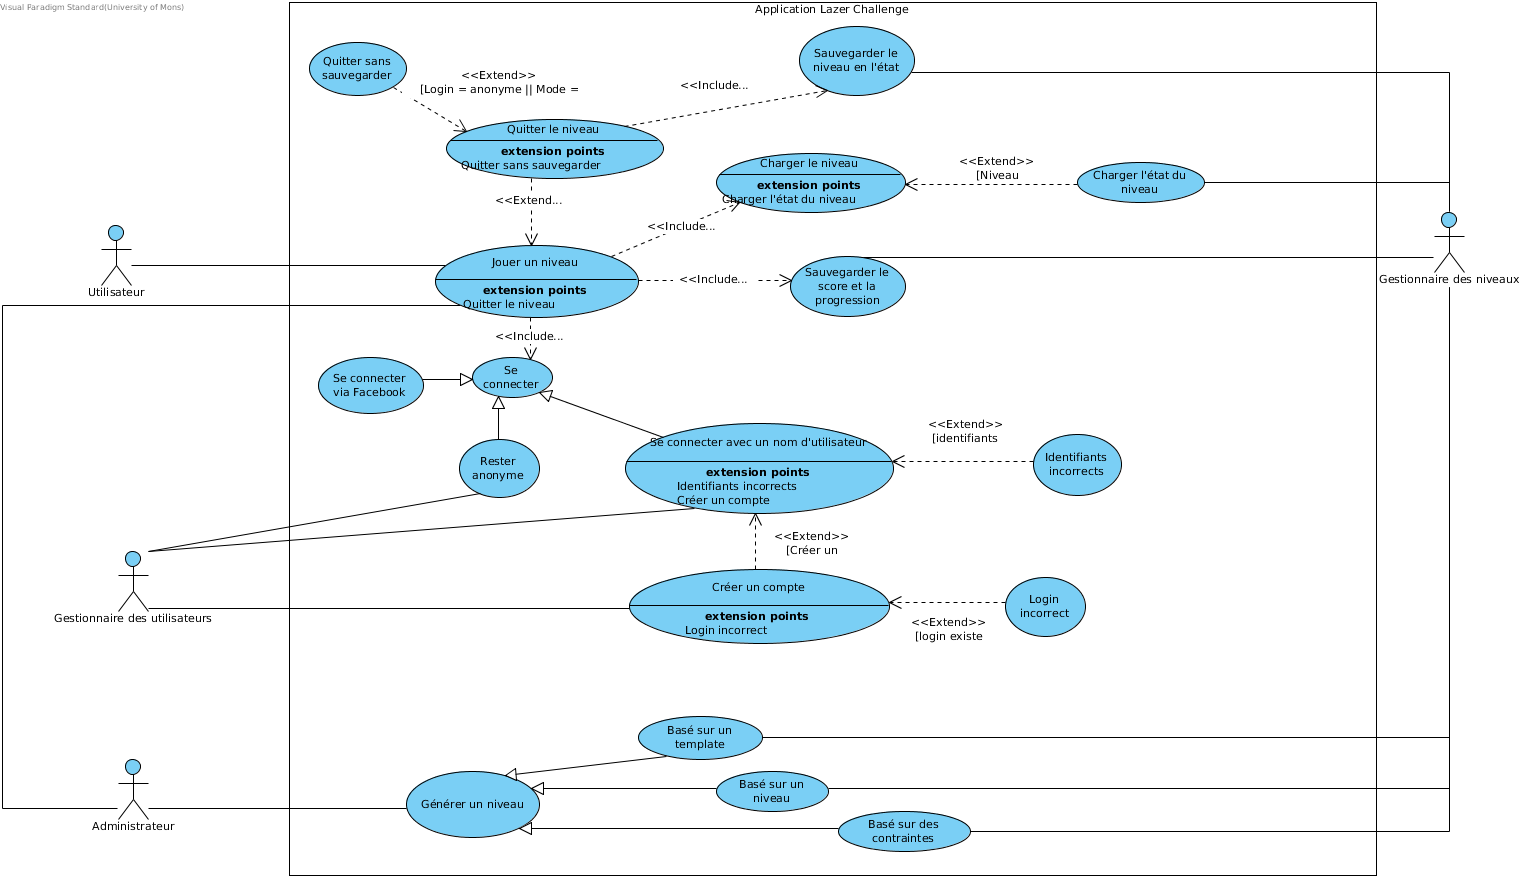
\includegraphics[scale=0.3]{../UseCase/UseCaseDiagram1.png}}

\textit{Voir Annexe 2,3 pour des PDF explicatifs }

\section{Diagramme d'état}

\centerline{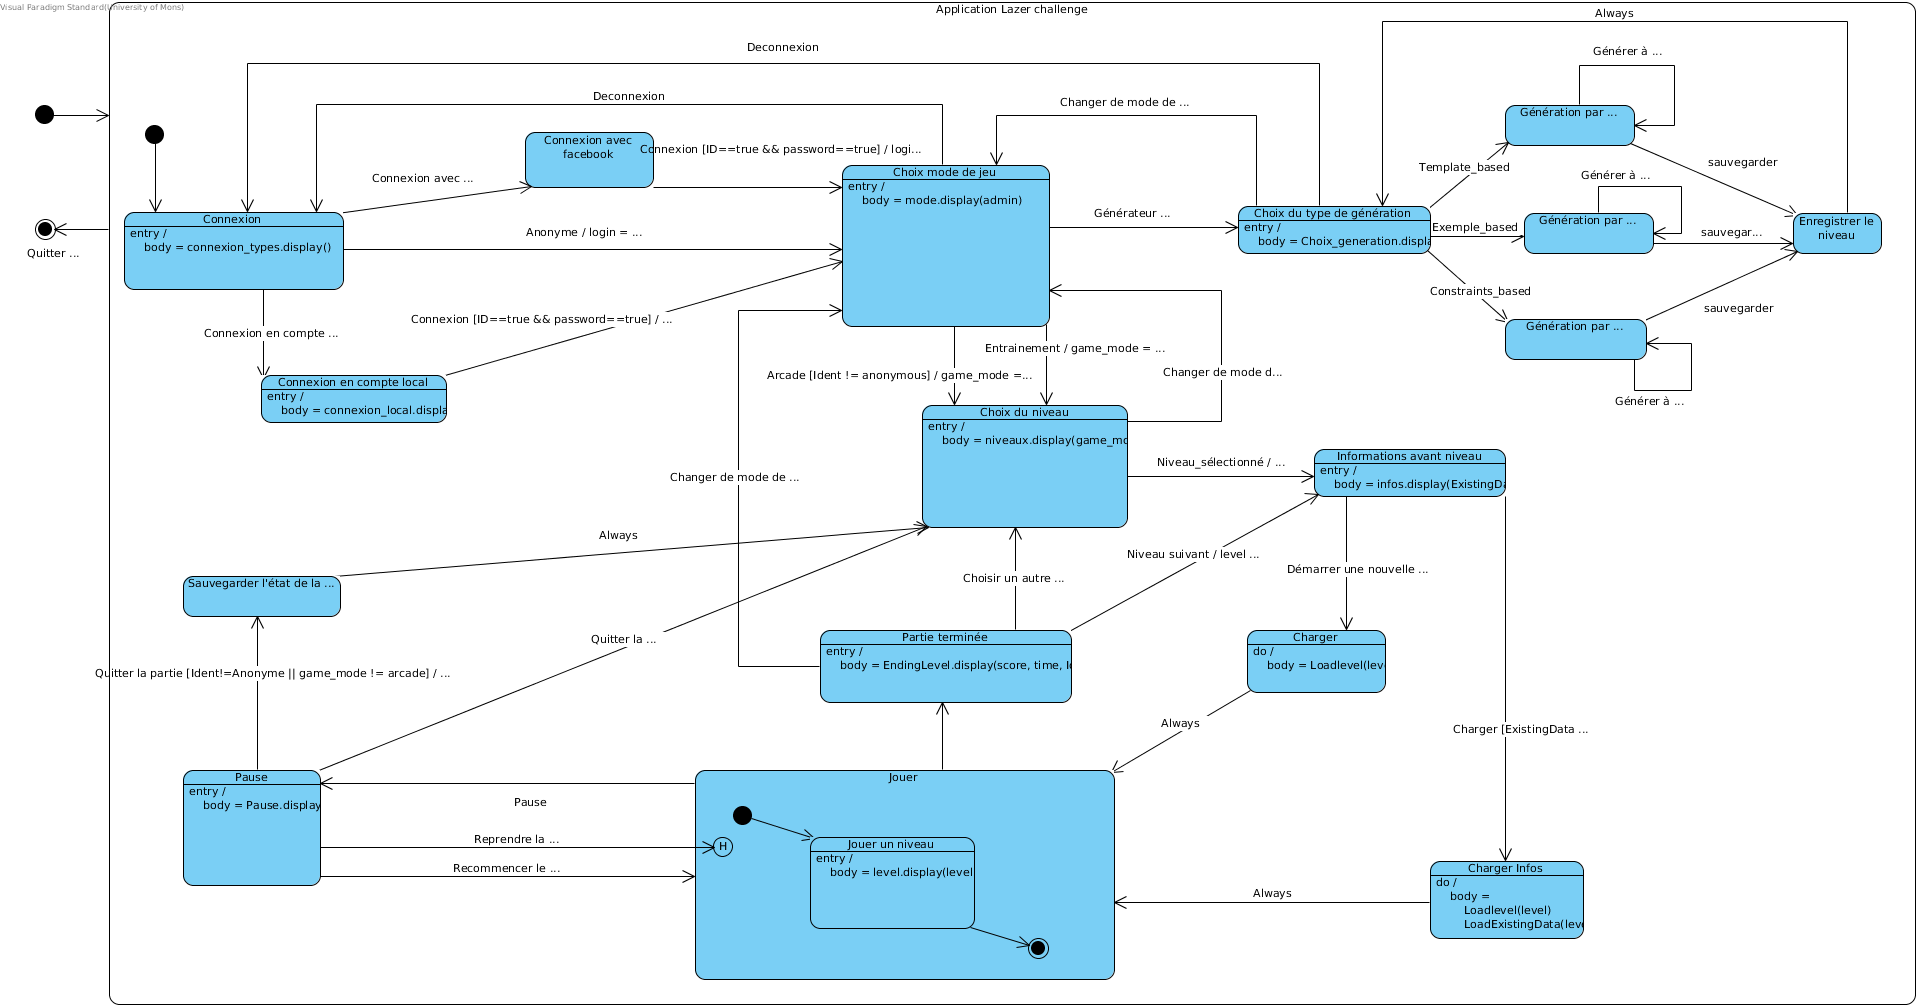
\includegraphics[scale=0.3]{../StateMachineDiagram/StateMachineDiagram1.png}}

\newpage

\section{Diagramme de classes}
\centerline{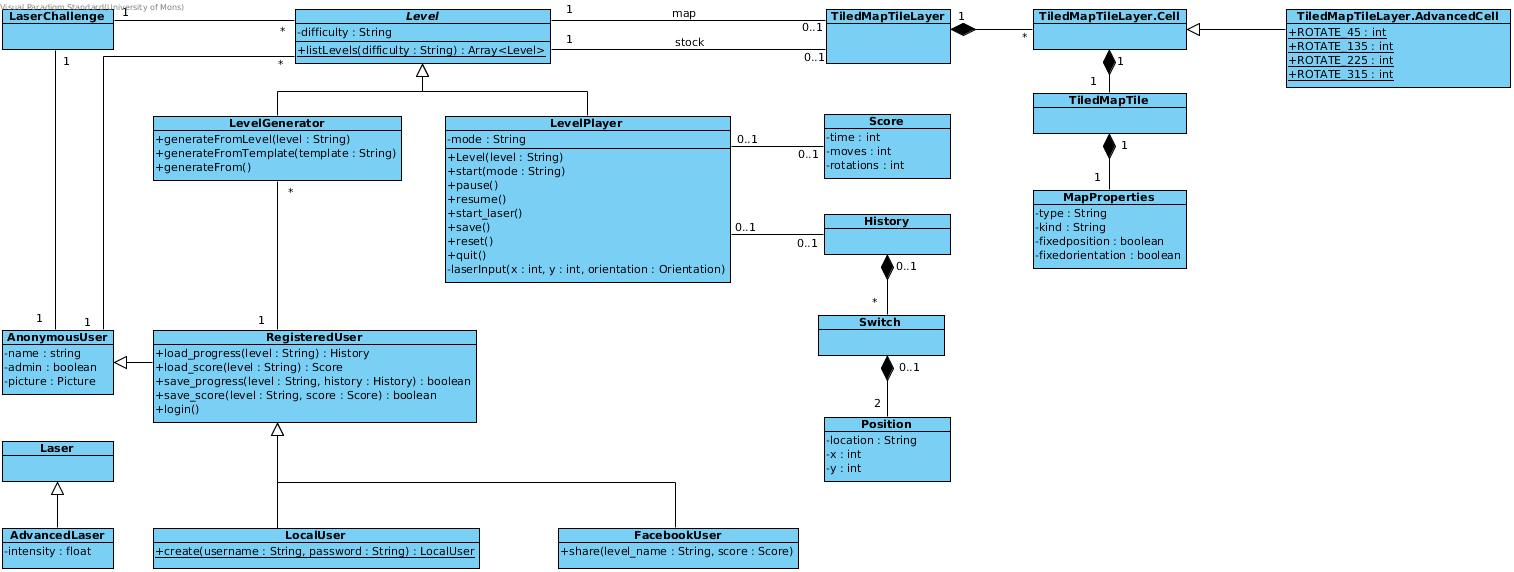
\includegraphics[scale=0.5]{../ClassDiagram/ClassDiagram.png}}

\newpage

\section{Diagrammes de séquences}
\textit{Figure 5.1 :Diagramme de séquence pour l'écran de connexion}

\centerline{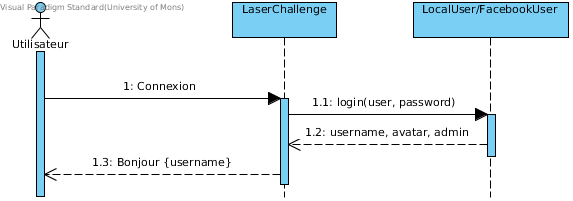
\includegraphics[scale=0.8]{../SequenceDiagram/Connexion.png}}

\textit{Figure 5.2 :Diagramme de séquence pour le choix des niveaux}

\centerline{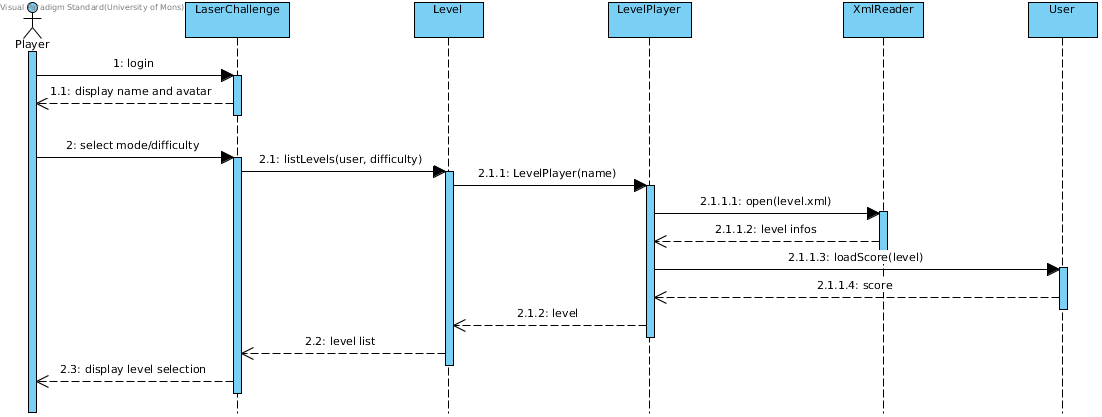
\includegraphics[scale=0.6]{../SequenceDiagram/LevelSelection.png}}

\textit{Figure 5.3 :Diagramme de séquence pour le commencement de la partie}

\centerline{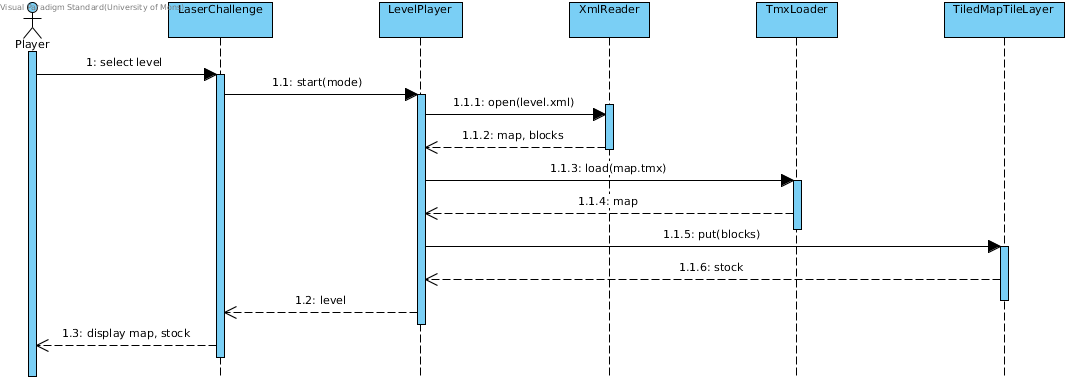
\includegraphics[scale=0.6]{../SequenceDiagram/LevelStart.png}}

\newpage

\section{Conclusion}
Notre but était d'obtenir une conception globale, cohérente et une structure solide pour la suite de notre projet. Comme précisé
dans notre Gantt, nous avons pris soin de travailler la maquette en parallèle de l'avancement de nos diagrammes. Tout ceci a pu être réalisé
grâce aux connaissances acquises au cours théorique ``Génie logiciel'' de Mr.Mens ainsi que celles acquises lors des séances d'exercices sous 
la direction de Mr.Devillez.



\end{document}
